%%% Local Variables:
%%% coding: utf-8
%%% mode: latex
%%% TeX-engine: xetex
%%% End:
\documentclass[12pt,a4paper, ngerman, oneside]{scrartcl}
\usepackage[ngerman]{babel}
\usepackage[utf8]{inputenc}
\usepackage{ucs}
\usepackage{amsmath}
\usepackage{amsfonts}
\usepackage{amssymb}
\usepackage{graphics}
\usepackage{paralist}
\usepackage{wrapfig}
\usepackage[linkcolor=black]{hyperref}
\usepackage{listings} \lstset{numbers=left, numberstyle=\tiny, numbersep=5pt} \lstset{language=Java}
%% Grafiken
\usepackage[pdftex]{graphicx}
\usepackage{epsfig}
\hypersetup{%
  colorlinks=true,
}

\newcommand\blfootnote[1]{%
  \begingroup
  \renewcommand\thefootnote{}\footnote{#1}%
  \addtocounter{footnote}{-1}%
  \endgroup
}
\hypersetup{
  pdfborder = {0 0 0},
  urlbordercolor = {0 0 0},
  colorlinks = true,
  linkcolor = black,
  citecolor = black,
  filecolor = black,
  urlcolor  = black
}
% Variablen
% siehe http://tex.stackexchange.com/a/290504 option 4
\def\Tiles/{8}
\def\Rundenlimit/{20}
\def\PointsPerTile/{7}
\def\PointsPerPassenger/{7}
\def\FieldsPerTile/{20}
\def\Passagiere/{5}

\newcommand{\fieldGraphic}[1]{%
\begin{wrapfigure}{r}{0.15\textwidth}%
  \includegraphics[width=0.15\textwidth]{bilder/#1}%
\end{wrapfigure}%
}

\sloppy
\hyphenpenalty=100000

\usepackage{fontspec}
\setromanfont{Merriweather}
\setsansfont{Lato}
\renewcommand{\normalsize}{\fontsize{12}{18}\selectfont}


\titlehead{\centering
\includegraphics[width=3.5cm]{bilder/logo.png}}
\subject{Software-Challenge 2017}
\title{Spielregeln}
\subtitle{Mississippi Queen}
\date{Stand: \today}


\begin{document}
\maketitle
%\begin{figure}[!htbp]
%  \centering
%  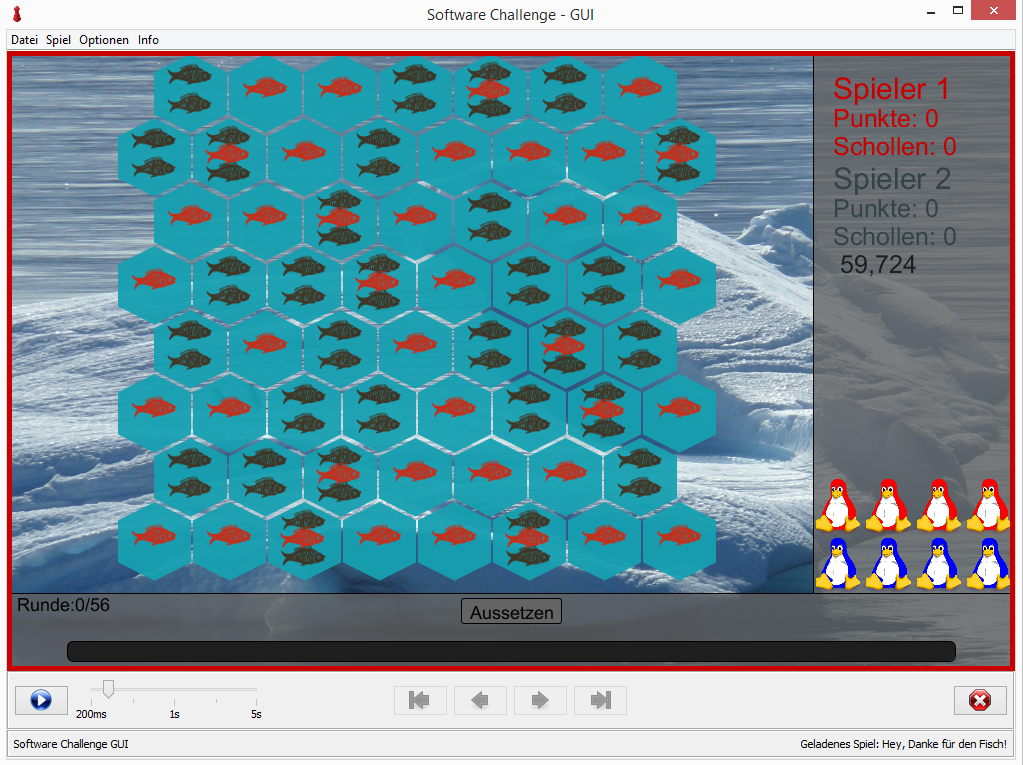
\includegraphics[width=\linewidth]{bilder/gui.png}
%\end{figure}
\vspace*{\fill}

\newpage
\tableofcontents
\thispagestyle{empty}
\newpage
\setcounter{page}{1}

\section{Einleitung}

In dieser Anleitung werden die Elemente und Regeln des Spiels Mississippi Queen
der Software-Challenge 2017 erläutert. Bei Mississippi Queen versuchen zwei
Spieler, durch abwechselndes setzen von Raddampfern schnellstmöglich einen Fluss
bis zum Ziel entlangzufahren und dabei zwei Passagiere mitzunehmen. Der Spieler,
der das Ziel mit zwei Passagieren an Bord zuerst erreicht, gewinnt das Spiel.


\section{Das Spielbrett}

Ein Ausschnitt des Spielbretts ist im Titelbild zu sehen. Es besteht aus \Tiles/
Spielsegmenten. Mit jeweils \FieldsPerTile/ Feldern. Am Anfang ist das nur das
Startsegment und ein darauf folgendes Segment aufgedeckt. Sobald ein Spieler das
letzte aufgedeckte Segment betritt, wird ein neues dahinter zufällig links,
rechts oder mittig angebaut. Dies geschieht solange, bis alle \Tiles/ Segmente
aufgedeckt wurden. Das letzte Segment ist das Zielsegment (TODO Graphik einfügen
darin Zielfelder markieren). Segmente die schon von allen Spielern betreten und
wieder verlassen wurden, werden vom Spielplan entfernt, auch wenn sich darauf
noch Passagiere befinden.

Die Spielsegmente enthalten zufällig verteilt verschiedene Arten von Feldern.
Neben Wasserfeldern, Inseln, Sandbänken und Baumstämmen gibt es pro Spiel
insgesamt \Passagiere/ Passagierfelder.


\subsection{\label{water}Das Wasserfeld (WATER)}

\fieldGraphic{wasser}

Das Wasserfeld (WATER) kann ganz normal befahren werden. Auf ein zum Spieler in
der aktuellen Bewegungsrichtung benachbartes Wasserfeld ziehen kostet einen
Geschwindigkeitspunkt.


\subsection{\label{island}Das Inselfeld (BLOCKED)}

\fieldGraphic{insel}

Das Inselfeld (BLOCKED) kann nicht überquert werden. Muss ein Spieler wegen zu
hoher Geschwindigkeit und zu wenig Kohlevorräten auf ein Inselfeld ziehen, hat
er das Spiel verloren.


\subsection{\label{passenger}Das Passagierfeld in Richtung $i$ (PASSENGER$i$)}

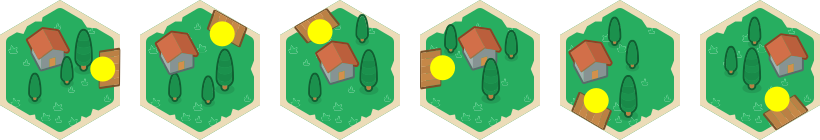
\includegraphics[width=\textwidth]{bilder/passagier}

Das Passagierfeld mit Anleger in Richtung $i$ enthält einen Passagier, der am
entsprechenden Anleger abgeholt werden kann. Um den Passagier abzuholen, muss
man auf dem Feld, welches zum Passagierfeld in Richtung des Anlegers benachbart
liegt, mit Geschwindigkeit 1 den Zug beenden. Es verwandelt sich in ein normales
Inselfeld, sobald der Passagier abgeholt wurde (siehe Inselfeld, \ref{island}).


\subsection{\label{goal}Das Zielfeld (GOAL)}

\fieldGraphic{ziel}

Das Zielfeld ist ein Feld, dass erreicht werden kann, um das Spiel zu gewinnen.
Das Zielfeld muss mit Geschwindigkeit 1 erreicht werden und der Zug muss auf dem
Zielfeld beendet werden. Es reicht nicht, auf das Zielfeld zu ziehen und dann
die Geschwindigkeit auf 1 zu reduzieren. Weiterhin müssen sich zwei Passagiere
an Bord befinden.


\subsection{\label{sandbank}Die Sandbank (SANDBANK)}

\fieldGraphic{sandbank}

Eine Sandbank bringt ein Schiff in der Bewegung zum halten, sollte man darauf
fahren. D.h. wenn ein Spieler auf eine Sandbank fährt, beendet dies seinen Zug
und setzt seine Geschwindigkeit auf 1. Es kann im nächsten Zug nur rückwärts
oder vorwärts mit der Bewegungsrichtung, mit der das Feld betreten wurde, wieder
verlassen werden. Verlässt man es Rückwärts, kostet dies zusätzlich eine
Kohleeinheit. Auf einer Sandbank kann nicht gedreht werden und ein Spieler, der
sich darauf befindet, kann nicht abgedrängt werden.


\subsection{Das Baumstammfeld (LOG)}

\fieldGraphic{baumstaemme}

Das ziehen in ein Baumstammfeld kostet die doppelte Anzahl an Bewegungspunkten,
also zwei Bewegungspunkte statt einem. Außerdem wird die Geschwindigkeit eines
Schiffes, welches ein Baumstammfeld durchquert nach dem Zug um 1 verringert.
Sind nicht genug Bewegungspunkte vorhanden, kann es nicht überquert werden. Das
Abdrängen in ein Baumstammfeld kostet einen zusätzlichen Bewegungspunkt.


\section{Spielablauf}

Beide Spieler starten mit Geschwindigkeit 1 und 6 Kohleeinheiten und ziehen dann
abwechselnd. Ein Zug besteht aus mehreren Aktionen. In allen Aktionen müssen
(falls der Zug nicht auf einer Sandbank endet) insgesamt alle Bewegungspunkte
(bestimmt durch die Geschwindigkeit des Schiffes) verbraucht werden. Die
verschiedenen Aktionen sind:


\subsection{\label{acceleration}Beschleunigungsaktion}

Kann nur als erste Aktion ausgeführt werden. Die Beschleunigung um eine
Geschwindigkeitseinheit ist frei, jede Beschleunigung um mehr als 1 kostet für
jeden weiteren Geschwindigkeitspunkt eine Kohleeinheit. Die
Höchstgeschwindigkeit ist 6, die niedrigste ist 1. Eine Beschleunigungsaktion um
0 ist ungültig. Möchte ein Spieler beispielsweise mit einer aktuellen
Geschwindigkeit von 2 auf Geschwindigkeit 4 beschleunigen, kostet dies eine
Kohleeinheit.

Auf gleiche weise kann auch abgebremst, also die Geschwindigkeit verringert
werden. Dies wird der Einfachheit halber als Beschleunigungsaktion mit negativer
Beschleunigung behandelt.


\subsection{\label{turn}Drehaktion}

Eine Drehaktion im Zug des Spielers um eine Einheit ist frei (Ausnahme
Abdrängen, siehe \ref{push}). Jede weitere Drehung erfordert eine Kohleeinheit.
Es kann sich nicht auf Sandbänken gedreht werden.


\subsection{\label{push}Abdrängaktion}

Zieht ein Spieler auf ein Feld, auf dem sich der gegnerische Spieler befindet,
muss darauf eine Abdrängaktion folgen. Ein Spieler kann den Gegner auf ein
beliebiges, angrenzendes, nicht direkt hinter den Spieler liegendes, begehbares
Feld abdrängen (\label{passierbar}Wasserfelder, Sändbänke und Baumstammfelder
gelten als begehbar). Eine Abdrängaktion kostet einen Bewegungspunkt, zwei,
falls auf ein Baumstammfeld abgedrängt wird. Es darf nicht von einer Sandbank
aus abgedrängt werden. Der abgedrängte Spieler bekommt eine zusätzliche freie
Drehung für seinen nächsten Zug. Wurde der Spieler auf eine Sandbank abgedrängt,
entfällt diese freie Drehung und die Geschwindigkeit des abgedrängten Spielers
wird auf 1 reduziert.

\subsection{\label{step}Bewegungsaktion}

Eine Bewegungsaktion erfolgt in die derzeitige Richtung des Schiffes des
Spielers. Sie kann nur über und auf passierbare (siehe \ref{passierbar}) Felder
erfolgen. Sie darf auf dem Feld des Gegners oder eine Sandbank enden, aber
niemals durch ein vom Gegner besetztes Feld oder eine Sandbank gehen.

\section{Spielende}

Das Spiel endet, sobald ein Spieler mit 2 Passagieren ein Zielfeld erreicht hat,
sobald das Rundenlimit von \Rundenlimit/ Runden erreicht ist, ein Spieler
auf ein ungültiges Feld ziehen muss oder falls nach dem Zug des Spielers der
nicht Startspieler war ein Spieler vier oder mehr Spielsegmente zurückliegt.

Wird das Rundenlimit erreicht gewinnt der Spieler mit den meisten Punkten. Die
Punkte errechnen sich folgendermaßen:

\begin{itemize}
  \item Jeder eingesammelte Passagier bringt 5 Punkte
  \item Jedes überwundene Segment bringt 5 Punkte.
  \item Anhand der Position innerhalb eines Segments werden 0 bis 4 Punkte
    vergeben. (Ein Segment ist aufgeteilt in 5 Reihen. je weiter vorne man ist,
    desto mehr Punkte bekommt man TODO siehe Graphik).
\end{itemize}

Sollten beide Spieler gleich viele Punkte haben, gewinnt der Spieler, der mehr
Passagiere eingesammelt hat. Sollte auch diese Zahl gleich sein, endet das Spiel
unentschieden.

\section{Graphische Benutzeroberfläche}

TODO

\end{document}
